%!TEX root = main.tex
  \section{\change{Related Works\label{sec:relatedworks}}}
  % \subsection{Background and Motivation}
  \par \change{We will now describe past work in visual query systems and existing evaluation methods of visualization systems to provide background and motivation to our work.
  % Visual query systems enable users to directly search for visualizations matching certain patterns through an intuitive specification interface. Early work in this space focused on interfaces to search for time series with specific patterns.
  \par \emph{Visual query systems} (VQSs) is a term coined by Ryall et al. and Correll and Gleicher\cite{ryall2005querylines,correll2016semantics} to describe systems that enable analysts to directly search for time-series visualizations matching certain patterns through an intuitive specification interface. Examples of such systems} include TimeSearcher~\cite{Hochheiser2001,Hochheiser2004}, where the query specification mechanism is a rectangular box, with the tool filtering out all of the time series that does not pass through it, QuerySketch~\cite{wattenberg2001sketching} and Google Correlate~\cite{mohebbi2011google}, where the query is sketched as a pattern on canvas, with the tool filtering out all of the time series that have a different shape. Subsequent work recognized the ambiguity in sketching by studying how humans rank the similarity in patterns~\cite{Eichmann2015,correll2016semantics,Mannino2018} and improving the expressiveness of sketched queries through finer-grained specification interfaces and pattern-matching algorithms~\cite{ryall2005querylines,Holz2009}.
  %performed crowdsourced perceptual studies to understand how humans rank similarity in patterns subjectively
  % , including the use of soft constraints~\cite{ryall2005querylines} and implicit relaxed selection techniques~\cite{Holz2009}.
  % In addition to this ongoing work, recent work have also performed crowdsourced perceptual studies to understand how humans rank similarity in patterns subjectively~\cite{Eichmann2015,correll2016semantics,Mannino2018}.
  \par While these systems have been effective in controlled lab studies, they have never been designed and evaluated in-situ on multiple real-world use cases. Even when use cases were involved~\cite{Hochheiser2004,correll2016semantics}, the inclusion of these \change{case studies served as a post-hoc demonstrative case study that had} little influence on the major design decisions of the system. In the context of Munzner's nested model~\cite{munzner2009nested}, this \change{gap between research and adoption stems from} the common ``downstream threat'' of jumping prematurely into the deep levels of \textit{encoding, interaction, or algorithm design}, before a proper \textit{domain problem characterization} and \textit{data/operation abstraction design} is performed. In this work, we performed design studies~\cite{lam2012empirical,shneiderman2006strategies,Sedlmair2012} with three different subject areas for \textit{domain problem characterization}. Comparing and contrasting between the diverse set of questions, datasets, and challenges across these three use cases revealed new generalizable insights and enabled us to better understand how VQSs can be extended for novel and unforeseen use cases. Based on these findings, we developed a taxonomy for understanding the sensemaking process in VQSs as part of the \textit{data/operation abstraction design}. Finally, we validated the abstraction design with grounded evaluation~\cite{Plaisant2004,Isenberg2008}, where we invited participants to bring in their own datasets and research problems that they have a vested interest in to test our final deployed system. \change{Next, we will outline these two phases of our study, deferring details of the study procedures and protocols to the technical report.}%Next, we will describe these two phases of our study in more detail.
  %had a narrow objective and had 
  \begin{table}[h!]
    \vspace*{-10pt}
     \centering
     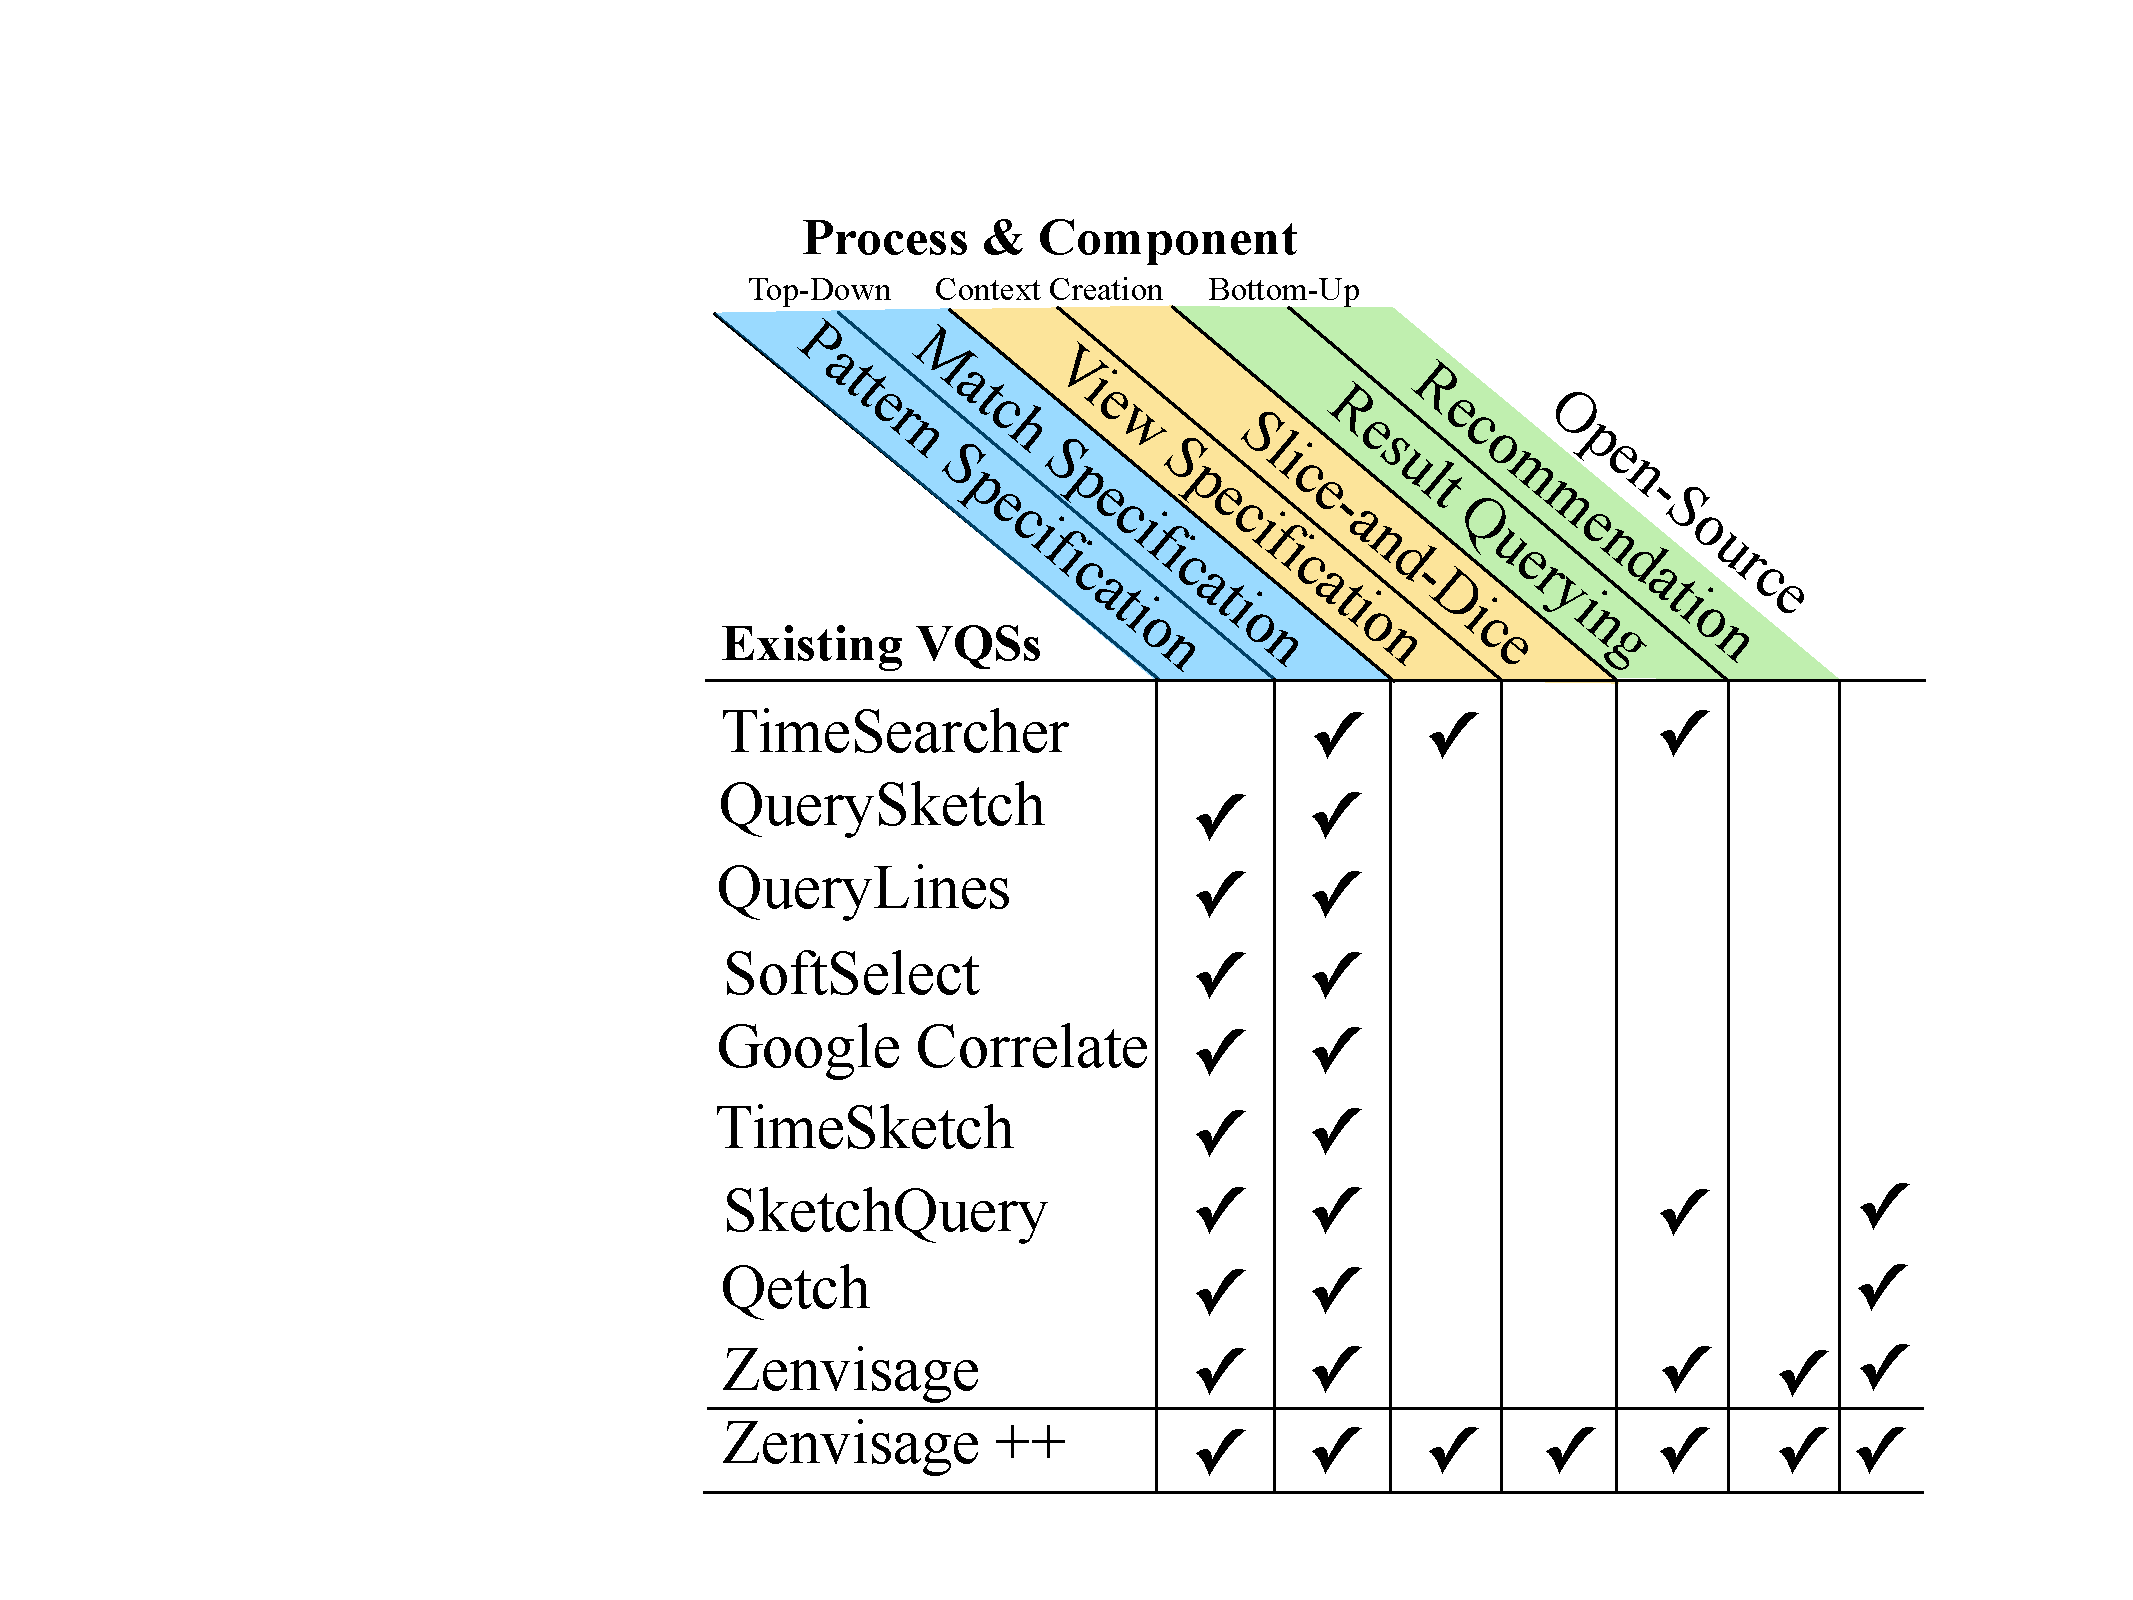
\includegraphics[width=0.8\linewidth]{figures/related_works_table.pdf}
     \caption{Table summarizing whether key functional components (columns) are covered by past systems (row), indicated by checked cells. Column header colors blue, orange, green represents three sensemaking process (top-down querying, search with context, and bottom-up querying) described in Section~\ref{sec:pd_findings}. The heavily-used, practical features in our study for context-creation and bottom-up inquiry is largely missing from prior VQSs.}
     \label{table:relatedwork}
     \vspace*{-15pt}
 \end{table}